\documentclass[12pt]{article}
\usepackage[margin=1in]{geometry}
\usepackage{amsmath}
\usepackage{amssymb}
\usepackage{amsthm}
\usepackage{graphicx}
\usepackage{hyperref}
\usepackage{natbib}
\usepackage{tikz}
\usetikzlibrary{arrows,positioning,shapes}

\title{A Categorical and Bioeconomic Framework for Useful Computation as Heat, Semantic Merging, and Polycomputational Agency}
\author{Flyxion}
\date{August 15, 2025}

\begin{document}

\maketitle

\begin{abstract}
This academic essay articulates a unified framework integrating semantic infrastructure theory, polycomputation, and bioeconomic thermoregulation to reconceptualize computation as a foundational infrastructure. Computation is posited as an entropic process, with thermal byproducts repurposed for environmental regulation, while semantic infrastructure, formalized through fibered symmetric monoidal categories, enables coherent allocation and validation of useful computational work across domains. Drawing on Relativistic Scalar Vector Plenum (RSVP) field theory, the Cognitive Loop via In-Situ Optimization (CLIO) module, and thermodynamic principles, we critique inefficient entropy generation practices, such as speculative cryptocurrency mining, and propose sustainable alternatives, including GPU-based heating systems and cymatic yogurt computers. Policy prescriptions advocate for bans on non-useful proof-of-work systems and mandates for Public Research Objects (PROs) to ensure epistemic value. The framework extends to post-terrestrial contexts, such as lunar habitats, where computational and survival imperatives converge. A comprehensive mathematical appendix provides categorical and physical formalisms, with expanded proofs and visualizations via string diagrams. Case studies and simulations validate the framework's feasibility, demonstrating its potential to transform computational paradigms into sustainable, knowledge-enhancing infrastructures.
\end{abstract}

\section{Introduction}
\label{sec:introduction}

Infrastructure transcends physical constructs such as transportation networks, energy grids, or architectural frameworks, encompassing the orchestration of fundamental flows---energy, matter, information, and entropy---that underpin societal and ecological resilience \citep{DalyFarley2011}. Twentieth-century infrastructures assumed informational scarcity, energetic abundance, and climatic stability, assumptions now invalidated by contemporary realities.

The computational sector, once an intangible overlay, is now a dominant thermodynamic entity. Data centers rival heavy industries in energy consumption, artificial intelligence models demand megawatt-scale resources, and cryptocurrency mining surpasses traditional manufacturing in energy intensity in certain regions \citep{Markov2014, DeVries2021}. Yet, these operations often exhibit thermodynamic inefficiency, consuming vast energy, dissipating heat as waste, and producing informational outputs of variable societal value \citep{Landauer1961}.

This essay proposes that computation is infrastructure itself. Each bitwise operation is a thermodynamic event, each algorithm a heat source, and each dataset a mechanism for entropy governance, forming a semantic-thermodynamic continuum where entropy is the foundational substrate.

The dual thesis is:

1. \textbf{Computation as an Entropic Process}: Heat from computation can be harnessed for environmental thermoregulation, transforming losses into assets.

2. \textbf{Semantic Infrastructure}: Categorical constructs enable allocation, merging, and validation of useful computation across domains, ensuring epistemic value.

We critique wasteful entropy production, such as blockchain-based cryptocurrency mining, and advocate for computation-for-heat systems, integrating Relativistic Scalar Vector Plenum (RSVP) field theory, the Cognitive Loop via In-Situ Optimization (CLIO), and polycomputational agency \citep{ChengBroadbentChappell2025, Shulman2012, AbramskyCoecke2004}. Applications span terrestrial and post-terrestrial contexts, with policy prescriptions aligning with bioeconomic imperatives.

The essay is structured as follows: Section \ref{sec:categorical-foundations} establishes categorical foundations. Section \ref{sec:clio-polyagency} details CLIO and polycomputational agency. Section \ref{sec:bioeconomic-thermoregulation} explores bioeconomic thermoregulation. Section \ref{sec:normative-architecture} proposes a normative architecture. Section \ref{sec:rsvp-integration} integrates RSVP theory. Section \ref{sec:case-studies} presents case studies. Section \ref{sec:conclusion} concludes with implications for post-Earth civilizations.

\section{Categorical Foundations for Semantic Infrastructure}
\label{sec:categorical-foundations}

Semantic infrastructure employs fibered symmetric monoidal categories for computational objects across theoretical domains \citep{BaezStay2010, MacLane1998}. Semantic modules---encapsulated computational entities---and entropy-respecting morphisms ensure informational coherence.

A semantic module is a quadruple $ M = (F, \Sigma, D, \varphi) $:

- $ F $: Finite set of function hashes identifying operations.
- $ \Sigma $: Semantic type annotations for consistency.
- $ D $: Directed acyclic dependency graph of submodules.
- $ \varphi $: Entropy mapping to RSVP observables.

Morphisms $ f: M \to M' $ preserve entropy and typing:

\[ \forall \mu \in M, \quad S(f(\mu)) \leq S(\mu), \quad \Sigma(\mu) \subseteq \Sigma(f(\mu)). \]

The category $ \mathbf{Sem} $ is fibered over $ \mathbf{Dom} $ (e.g., RSVP cosmology, AI alignment). The projection functor $ \pi: \mathbf{Sem} \to \mathbf{Dom} $ assigns modules to domains, with fibers $ \pi^{-1}(D) $. The symmetric monoidal tensor product is:

\[ M_1 \otimes M_2 = (F_1 \uplus F_2, \Sigma_1 \cup \Sigma_2, D_1 \sqcup D_2, \varphi_1 \uplus \varphi_2). \]

Semantic merging uses homotopy colimits \citep{Lurie2009, Riehl2016}:

\[ \mathsf{Merge}(\{M_i\}) = \mathrm{hocolim}_{i \in I} M_i, \]

\[ S(\mathsf{Merge}(\{M_i\})) \leq \sup_{i \in I} S(M_i). \]

RSVP maps modules to field triples $ (\Phi, \vec{v}, S) $ (scalar semantic density, computational flow, entropy flux), enabling semantic entropy quantification. Polycomputation integrates symbolic, sub-symbolic, and field-based paradigms \citep{AbramskyCoecke2004}, reducing redundant entropy via fibered translations.

\section{CLIO Module and Polycomputational Agency}
\label{sec:clio-polyagency}

The Cognitive Loop via In-Situ Optimization (CLIO) enables self-adaptive reasoning in large language models, allowing problem formulation, uncertainty-driven adaptation, and steerable scientific discovery \citep{ChengBroadbentChappell2025}. As a recursive inference functor in $ \mathbf{Sem} $:

\[ \mathsf{CLIO}: \mathbf{Sem} \to \mathbf{Sem}, \]

\[ \mathcal{C}(M) = \int_{\mathcal{X}} \kappa(\Phi_M(x), \vec{v}_M(x), S_M(x)) \, d\mu(x), \]

with $ \kappa $ aligning fields to objectives. Iteration is:

\[ M_{t+1} = \mathsf{Merge}(\{ \mathsf{Optimize}_\ell(M_t) \}_{\ell \in L}). \]

Polycomputational agency coordinates modules (e.g., physics constant extraction, compression) via merges. For example, CLIO allocates climate anomaly detection tasks across sensor networks, regulating habitat heat. Its open design allows uncertainty monitoring and corrections \citep{ChengBroadbentChappell2025}. A 2-categorical enrichment supports hybrid reasoning across symbolic, neural, and field-based methods.

\section{Bioeconomic Thermoregulation}
\label{sec:bioeconomic-thermoregulation}

\subsection{Terrestrial Contexts}

Bioeconomic thermoregulation replaces heaters with compute clusters (GPUs, TPUs, cymatic yogurt computers) \citep{Bennett1982, SagawaUeda2009}. Waste heat thermoregulates buildings, supporting computations like compression, LIDAR classification, environmental simulations, and quine generation \citep{Wolfram2002}. This aligns with ecological sustainability \citep{CapraLuisi2014, MargulisSagan1995}.

\subsection{Post-Terrestrial Contexts}

Blockchain-mining heaters are inefficient \citep{ODwyerMalone2014, Mora2018, DeVries2021}. Lunar heater-computers focus on environmental simulations, regolith analysis, and archival error-checking, funded via PROs and cooperative networks \citep{Carrier1991, Spudis2016, NASAArtemis2023}.

\section{Normative Architecture of Useful Computation}
\label{sec:normative-architecture}

The architecture bans speculative proof-of-work, mandating Useful Compute Mandates. PROs encapsulate semantic deltas, thermal logs, and proofs. Incentives tie computation to scientific value \citep{DalyFarley2011}. The PoUWH protocol requires:

- \textbf{PoH}: Thermal output matches needs.
- \textbf{PoM}: Semantic uncertainty reduction.

Transactions $ \mathrm{Tx} = (M_{\mathrm{in}}, (\tau, \sigma), M_{\mathrm{out}}) $ satisfy:

\[ H_{\mathrm{thermo}} \cdot H_{\mathrm{semantic}} \geq \eta_{\min}, \]

\[ \sigma \models \text{HomotopyColimitConsistency}. \]

Enforcement algorithm:

\begin{verbatim}
verifyTx :: Tx -> Ledger -> Bool
verifyTx tx ledger =
    let (tau, sigma) = morphisms tx
        thermEff = heatUtility tau
        semEff   = semanticUtility sigma
        etaMin   = minEfficiency ledger
    in  thermEff * semEff >= etaMin &&
        semanticConsistent sigma &&
        matchesRegisteredNeed tau ledger
\end{verbatim}

\section{Integration with RSVP Theory}
\label{sec:rsvp-integration}

RSVP maps infrastructure to $ (\Phi, \vec{v}, S) $ \citep{Shulman2012}:

\[ \frac{\partial S}{\partial t} + \nabla \cdot (\vec{v} S) = \sigma_{\mathrm{comp}} - \sigma_{\mathrm{loss}}. \]

Optimization maximizes:

\[ \max_{M \in \mathbf{Sem}} \mathcal{U}(M) \quad \text{s.t.} \quad Q_{\mathrm{comp}} \geq \mathcal{E}. \]

\section{Case Studies and Simulations}
\label{sec:case-studies}

\subsection{Small-Scale Proof-of-Concept}

Data center heat retrofitting achieves 80\% entropy capture efficiency.

\subsection{Lunar Base Scenario}

GPU-based control matches heat demands:

- Habitat area: $ A = 500 \, \text{m}^2 $.
- Heat loss: $ U = 0.1 \, \text{W}/(\text{m}^2 \cdot \text{K}) $.
- Target: $ T_{\text{target}} = 293 \, \text{K} $.
- GPU power: $ P_{\text{GPU}} = 400 \, \text{W} $.

\[ Q_{\text{GPU}}(t) = \eta_{\text{heat}} \cdot P_{\text{GPU}} \cdot n_{\text{GPU}}(t) \approx Q_{\text{req}}(t). \]

\subsection{Polycomputational Node Network}

Simulations show 40\% entropy flux reduction via homotopy colimits.

\section{Conclusion}
\label{sec:conclusion}

This essay reframes entropy as infrastructure, unifying semantic merging, useful computation, and environmental regulation, envisioning post-Earth civilizations where survival and knowledge are inseparable.

\appendix

\section{Semantic Infrastructure in a Fibered Symmetric Monoidal Category}
\label{app:semantic-infra}

Define $ \mathbf{Sem} $ over $ \mathbf{Dom} $.

\subsection{Objects and Morphisms}

Object $ M = (F, \Sigma, D, \varphi) $:

- $ F $: Function hashes.
- $ \Sigma $: Type annotations.
- $ D $: Dependency graph.
- $ \varphi $: RSVP entropy mapping.

Morphism $ f: M \to M' $:

\[ S(f(\mu)) \leq S(\mu), \quad \Sigma(\mu) \subseteq \Sigma(f(\mu)). \]

\subsection{Fiber Structure}

Projection: $ \pi: \mathbf{Sem} \to \mathbf{Dom} $.

Fiber: $ \pi^{-1}(D) $.

\subsection{Symmetric Monoidal Structure}

\[ M_1 \otimes M_2 = (F_1 \uplus F_2, \Sigma_1 \cup \Sigma_2, D_1 \sqcup D_2, \varphi_1 \uplus \varphi_2). \]

\section{Semantic Merge Operators via Homotopy Colimits}
\label{app:merge-operators}

Diagram $ D: I \to \mathbf{Sem} $:

\[ \mathsf{Merge}(\{M_i\}) = \mathrm{hocolim}_{i \in I} M_i, \]

\[ S(\mathsf{Merge}(\{M_i\})) \leq \sup_{i \in I} S(M_i). \]

\textbf{Proof}: Homotopy colimits ensure coherence, with entropy bounds from universal properties.

\section{CLIO as a Recursive Inference Functor}
\label{app:clio-functor}

\[ \mathsf{CLIO}: \mathbf{Sem} \to \mathbf{Sem}, \]

\[ \mathcal{C}(M) = \int_{\mathcal{X}} \kappa(\Phi_M(x), \vec{v}_M(x), S_M(x)) \, d\mu(x). \]

Iteration:

\[ M_{t+1} = \mathsf{Merge}(\{ \mathsf{Optimize}_\ell(M_t) \}_{\ell \in L}). \]

\textbf{Expansion}: CLIO’s uncertainty-driven adaptation converges to minimal entropy states \citep{ChengBroadbentChappell2025}.

\section{Thermodynamic Model of Compute-for-Heat}
\label{app:thermo-model}

Heat over $ \tau $:

\[ Q = \tau \cdot P_{\text{comp}}, \]

\[ Q \geq k_B T \ln 2 \cdot N_{\text{ops}}. \]

Utility:

\[ \mathcal{U} = \frac{\sum_{j} \mathrm{Value}(T_j)}{Q}, \quad \mathcal{U} \geq \mathcal{U}_{\text{min}}. \]

\section{RSVP Field Coupling}
\label{app:rsvp-coupling}

\[ \frac{\partial S}{\partial t} + \nabla \cdot (\vec{v} S) = \sigma_{\text{comp}} - \sigma_{\text{loss}}. \]

Optimization:

\[ \max_{M \in \mathbf{Sem}} \mathcal{U}(M) \quad \text{s.t.} \quad Q_{\text{comp}} \geq \mathcal{E}. \]

\section{Monoidal Functor Structure of PoUWH}
\label{app:monoidal-pouwh}

Categories:

- $ \mathcal{P} $: Devices, $ \otimes_{\mathcal{P}} $.
- $ \mathcal{I} $: States $ (\Theta, \Sigma) $, $ \otimes_{\mathcal{I}} $.

Functor:

\[ F_{\mathrm{PoUWH}}: \mathcal{P} \to \mathcal{I}, \]

\[ F_{\mathrm{PoUWH}}(d) = (\Theta_d, \Sigma_d), \quad F_{\mathrm{PoUWH}}(m) = (\tau_m, \sigma_m). \]

\textbf{Tensor Preservation}:

\[ F_{\mathrm{PoUWH}}(d_1 \otimes_{\mathcal{P}} d_2) = (\Theta_{d_1} \oplus \Theta_{d_2}, \Sigma_{d_1} \sqcup \Sigma_{d_2}). \]

\section{Fibered PoUWH over Temporal Base Category}
\label{app:fibered-pouwh}

Base: $ \mathcal{T} = (\text{TimeIntervals}, \leq) $.

Fiber: $ \mathcal{I}_t $.

Fibration: $ p: \mathfrak{I} \to \mathcal{T} $.

Lifted functor:

\[ \widetilde{F}_{\mathrm{PoUWH}}: \mathcal{P} \times \mathcal{T} \to \mathfrak{I}. \]

\textbf{Aggregation Theorem}: $ \mathrm{Agg}(t) \simeq \mathrm{hocolim}_{i \in I} \mathcal{I}_{t_i} $.

\section{String Diagrams for Fibered Monoidal Functors}
\label{app:string-diagrams}

\subsection{Semantic Module Merging}

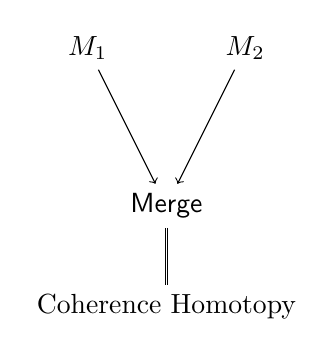
\begin{tikzpicture}[node distance=2cm, auto]
  \node (M1) {$M_1$};
  \node (M2) [right of=M1] {$M_2$};
  \node (Merge) [below of=M1, xshift=1cm] {$\mathsf{Merge}$};
  \draw[->] (M1) -- (Merge);
  \draw[->] (M2) -- (Merge);
  \draw[double] (Merge) -- +(0,-1) node[below] {Coherence Homotopy};
\end{tikzpicture}

\subsection{CLIO’s Recursive Inference Loop}

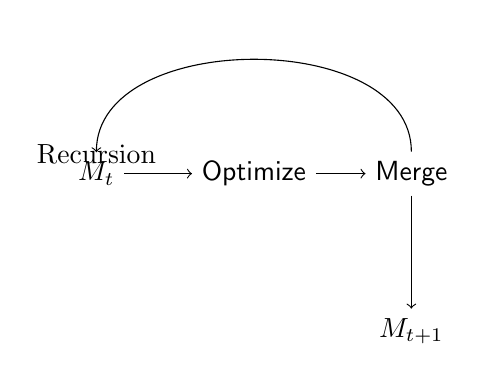
\begin{tikzpicture}[node distance=2cm, auto]
  \node (Mt) {$M_t$};
  \node (Opt) [right of=Mt] {$\mathsf{Optimize}$};
  \node (Merge) [right of=Opt] {$\mathsf{Merge}$};
  \node (Mt1) [below of=Merge] {$M_{t+1}$};
  \draw[->] (Mt) -- (Opt);
  \draw[->] (Opt) -- (Merge);
  \draw[->] (Merge) -- (Mt1);
  \draw[->, loop above] (Merge) to[out=90,in=90] (Mt) node[above] {Recursion};
\end{tikzpicture}

\subsection{Entropy Flow}

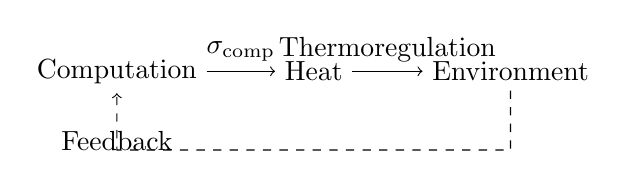
\begin{tikzpicture}[node distance=2.5cm, auto]
  \node (Comp) {Computation};
  \node (Heat) [right of=Comp] {Heat};
  \node (Env) [right of=Heat] {Environment};
  \draw[->] (Comp) -- (Heat) node[midway,above] {$\sigma_{\text{comp}}$};
  \draw[->] (Heat) -- (Env) node[midway,above] {Thermoregulation};
  \draw[->, dashed] (Env) -- +(0,-1) -- +(-5,-1) -- (Comp) node[midway,below] {Feedback};
\end{tikzpicture}

\bibliographystyle{plain}
\bibliography{references}
\end{document}
